\section*{Problem 1}
\addcontentsline{toc}{section}{Problem 1}

Let the random vector $(\alpha, \beta)$ is uniformely distributed in $\mathcal{G} = \{x^2 + y^2 < 1\quad y > 0 \}$, i.e.
\[
    f_{(\alpha, \beta)}(x, y) =
    \begin{cases}
        \text{const} & x, y \in \mathcal{G},    \\
        0            & x, y \notin \mathcal{G}.
    \end{cases}
\]

(a) Find the constant value.

(b) Find the probability density $f_\alpha(x)$ of the first component $\alpha$.

(c) Find the probability density of $\rho = \sqrt{\alpha^2 + \beta^2}$. Plot the function $f_\rho(t)$.

(d) Find the probability density of $\phi = \arccos(\alpha/\sqrt{\alpha^2 + \beta^2})$. Plot the function $f_\phi(t)$.

\subsection*{Solution (a)}

To find the constant value, we need to find the value of $c$ such that the integral of the function $f_{(\alpha, \beta)}(x, y)$ over the region $\mathcal{G}$ is equal to $1$.

\begin{equation}
    \int_{\mathcal{G}} f_{(\alpha, \beta)}(x, y) \, dx \, dy = 1
\end{equation}

\begin{equation}
    \int_{\mathcal{G}} c \cdot \, dx \, dy = 1
\end{equation}

\begin{equation}
    c \cdot  \int_{\mathcal{G}}\, dx \, dy = 1
\end{equation}

And because the integral $ \int_{\mathcal{G}}\, dx \, dy$ is equal
to the area of the region $\mathcal{G}$. So because the area of
a circle is $\pi r^2$ and we are taking only the upper half of the circle,
the area of the region $\mathcal{G}$ is $\pi \cdot 1^2 / 2 = \pi / 2$.

\begin{equation}
    c \cdot \frac{\pi}{2} = 1
\end{equation}

\begin{equation}
    c = \frac{2}{\pi}
\end{equation}

\subsection*{Solution (b)}

To find the probability density $f_\alpha(x)$ of the first component $\alpha$, we need to integrate the function $f_{(\alpha, \beta)}(x, y)$ over the second component $\beta$.

\begin{equation}
    f_\alpha(x) = \int_{-\infty}^{\infty} f_{(\alpha, \beta)}(x, y) \, dy
\end{equation}

We can notice that for $|x| > 1$, the function $f_{(\alpha, \beta)}(x, y)$
is equal to $0$, so we only need to take $|x| \leq 1$.
And because the $y$ component is always positive, we can integrate from $0$ to $\sqrt{1 - x^2}$.

\begin{equation}
    f_\alpha(x) = \int_{0}^{\sqrt{1 - x^2}} \frac{2}{\pi} \, dy
\end{equation}

Solving the integral, we get:

\begin{equation}
    f_\alpha(x) = \frac{2}{\pi} \cdot \sqrt{1 - x^2}
\end{equation}

So the probability density of the first component $\alpha$ is:

\begin{equation}
    f_\alpha(x) =
    \begin{cases}
        \frac{2}{\pi} \cdot \sqrt{1 - x^2} & |x| \leq 1, \\
        0                                  & |x| > 1.
    \end{cases}
\end{equation}

\subsection*{Solution (c)}

The random variable \(\rho\) represents the distance from the origin to the point \((\alpha, \beta)\) in the upper half of the unit circle. The cumulative distribution function (CDF) of \(\rho\) is the probability that \(\rho\) is less than or equal to a certain value \(r\), which is the area of the upper half of the circle with radius \(r\) divided by the total area of the unit circle. For \(0 \leq r \leq 1\), this area is \(\frac{1}{2} \pi r^2\). Therefore, the CDF of \(\rho\) is:

\[ F_{\rho}(r) = \frac{\frac{1}{2} \pi r^2}{\frac{1}{2} \pi} = r^2 \]

The probability density function (PDF) is the derivative of the CDF. Thus,

\[ f_{\rho}(r) = \frac{d}{dr} F_{\rho}(r) = 2r \]

So the probability density of \(\rho\) is:

\begin{equation}
    f_\rho(r) =
    \begin{cases}
        2r & 0 \leq r \leq 1,         \\
        0  & r < 0 \text{ or } r > 1.
    \end{cases}
\end{equation}

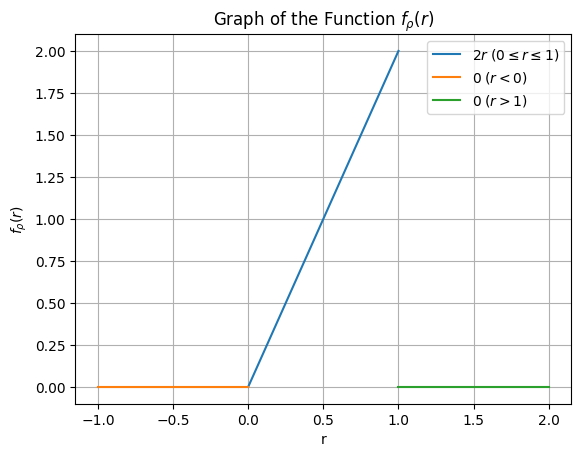
\includegraphics[width=\textwidth]{images/p1.png}

\subsection*{Solution (d)}

We can notice that $a$ is the adjacent side of a right triangle
with hypotenuse $\rho = \sqrt{\alpha^2 + \beta^2}$ and opposite
side $\beta$. So we can use the definition of cosine:

\begin{equation}
    \cos(\phi)  \frac{\alpha}{\sqrt{\alpha^2 + \beta^2}}
\end{equation}

So then:

\begin{equation}
    \arccos(\frac{\alpha}{\sqrt{\alpha^2 + \beta^2}}) = \arccos(\cos(\phi)) = \phi
\end{equation}

The the problem is equivalent to finding the probability density of $\phi$,
where $\phi$ is the angle between the vector $(\alpha, \beta)$ and the $x$ axis.

Let's find the CDF of $\phi$. The CDF of $\phi$ is the probability that
$\phi$ is less than or equal to a certain value $\theta$, which is the
area of the region $\mathcal{G}_\theta$ divided by the total area of
the region $\mathcal{G}$. The region $\mathcal{G}_\theta$ is the regio
n between the $x$ axis and the line that makes an angle $\theta$ with
the $x$ axis. The total area of the region $\mathcal{G}$ is $\pi / 2$.

To find the area of the region $\mathcal{G}_\theta$, we can just
find the area of a sector of a circle with radius $r$ and angle $\theta$,
this area can be easily calculated as $\frac{1}{2} r^2 \theta$.

So the CDF of $\phi$ is:

\begin{equation}
    F_\phi(\theta) = \frac{\frac{1}{2} \theta}{\frac{1}{2} \pi} = \frac{\theta}{\pi}
\end{equation}

The PDF of $\phi$ is the derivative of the CDF. So:

\begin{equation}
    f_\phi(\theta) = \frac{d}{d\theta} F_\phi(\theta) = \frac{1}{\pi}
\end{equation}

Then because the angle $\phi$ is between $0$ and $\pi$, and for
the other values the PDF is $0$, we get:

\begin{equation}
    f_\phi(\theta) =
    \begin{cases}
        \frac{1}{\pi} & 0 \leq \theta \leq \pi,              \\
        0             & \theta < 0 \text{ or } \theta > \pi.
    \end{cases}
\end{equation}

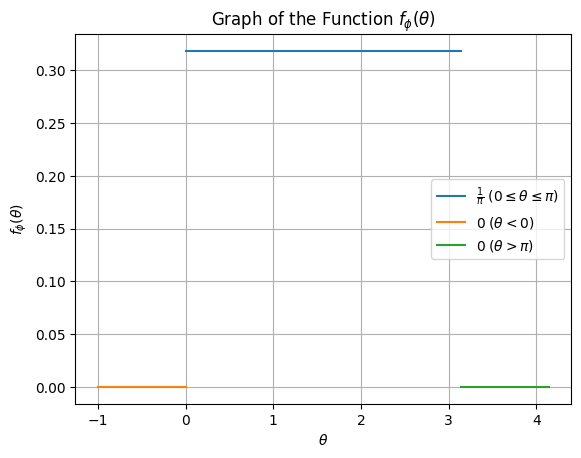
\includegraphics[width=\textwidth]{images/p2.png}